\documentclass[11pt,a4paper]{article}
\usepackage[utf8]{inputenc}
\usepackage[portuguese]{babel}
\usepackage{amsmath}
\usepackage{amsfonts}
\usepackage{amssymb}
\usepackage{graphicx}
\usepackage{float}
\usepackage{geometry}
\usepackage{hyperref}
\usepackage{caption}
\usepackage{subcaption}

\geometry{margin=2.5cm}

\title{Comparação de Estratégias do Cálculo das Equações do Fermat}
\author{Análise de Performance e Precisão}
\date{\today}

\begin{document}

\maketitle

\section{Introdução}

\subsection{Cenário de Análise}

O presente estudo analisa um cenário SAR bistático composto por um alvo (target) e dois radares separados: um transmissor (Tx) e um receptor (Rx), operando sobre uma superfície plana. A Figura \ref{fig:cenario} ilustra a configuração geométrica fundamental do sistema.

\begin{figure}[H]
\centering
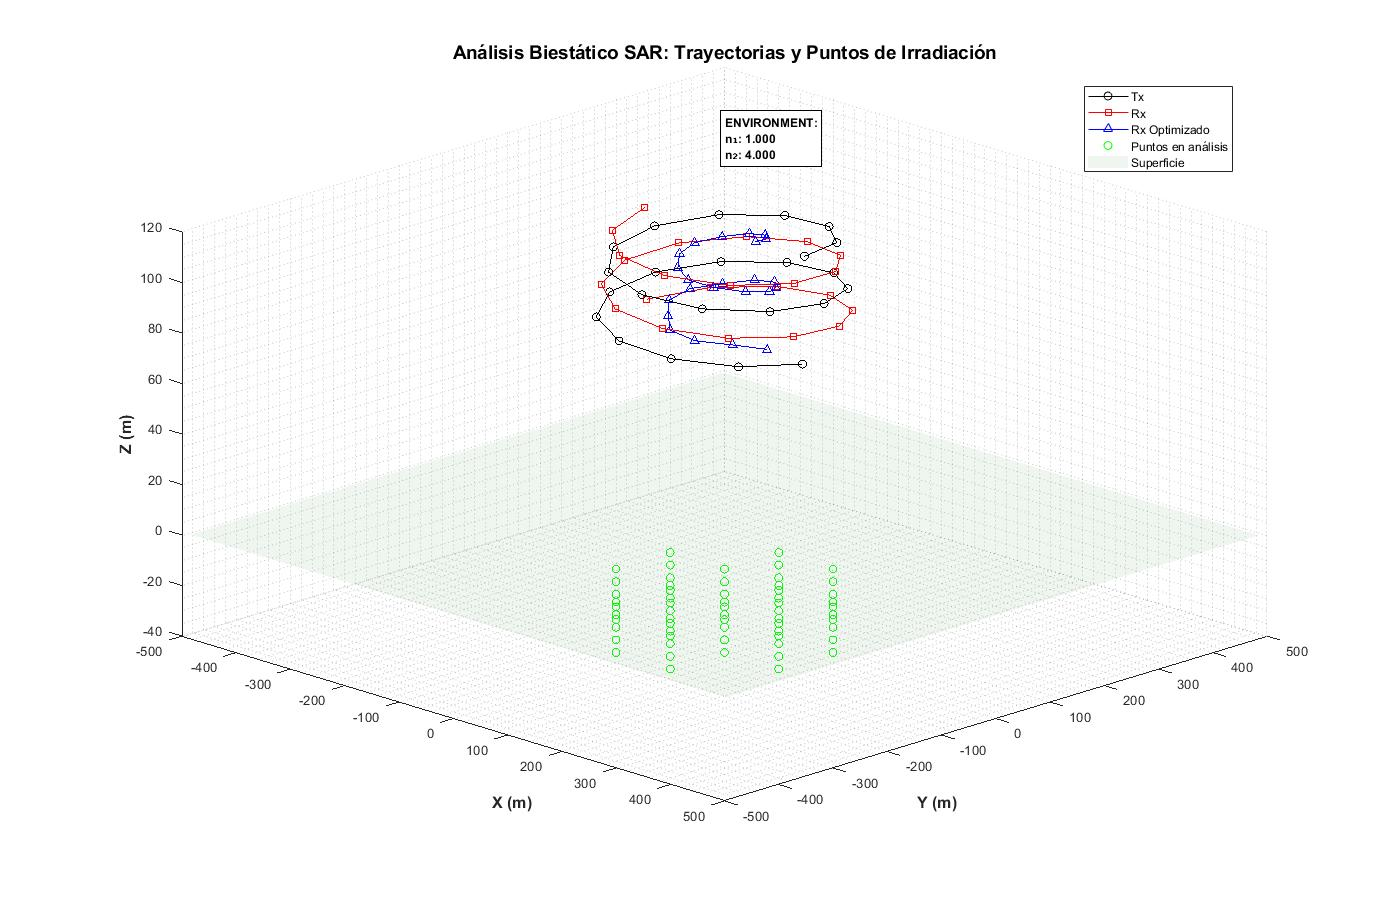
\includegraphics[width=0.8\textwidth]{../cenario.png}
\caption{Cenário SAR bistático analisado, mostrando a disposição espacial do transmissor (Tx), receptor (Rx), alvo (target) e superfície plana. Esta configuração serve como base para a análise comparativa das estratégias de cálculo das equações do Fermat.}
\label{fig:cenario}
\end{figure}

Nesta configuração, a onda eletromagnética emitida pelo transmissor pode seguir diferentes trajetórias até o receptor:
\begin{itemize}
\item \textbf{Reflexão direta}: Do transmissor para o alvo, refletindo diretamente para o receptor
\item \textbf{Reflexão na superfície}: Do transmissor para a superfície, refletindo para o alvo e posteriormente para o receptor
\item \textbf{Refração}: Trajetórias que envolvem mudanças de meio, considerando diferentes velocidades de propagação
\end{itemize}

\subsection{Fundamentação Teórica}

O princípio de Fermat estabelece que a luz percorre o caminho que minimiza o tempo de viagem entre dois pontos. Em sistemas SAR bistáticos, este princípio é fundamental para determinar os pontos de reflexão e refração na superfície terrestre. Este documento apresenta uma análise comparativa de duas estratégias distintas para o cálculo das equações do Fermat: uma abordagem iterativa de alta precisão e uma estratégia vetorizada eficiente.

\section{Fundamentação Matemática}

\subsection{Princípio de Fermat}

O princípio de Fermat pode ser expresso matematicamente como a minimização do tempo total de percurso da onda eletromagnética:

\begin{equation}
T_{total} = \int_{caminho} \frac{ds}{v(s)}
\end{equation}

onde $ds$ é um elemento infinitesimal do caminho e $v(s)$ é a velocidade local da onda.

Para cenários bistáticos com reflexão e refração, temos três tipos de trajetórias:

\begin{enumerate}
\item \textbf{Reflexão}: $T_{refl} = \frac{||\vec{Tx} - \vec{S}||}{v_1} + \frac{||\vec{S} - \vec{Rx}||}{v_1}$
\item \textbf{Refração (ida)}: $T_{refr,ida} = \frac{||\vec{Tx} - \vec{Q}||}{v_1} + \frac{||\vec{Q} - \vec{P}||}{v_2}$
\item \textbf{Refração (volta)}: $T_{refr,volta} = \frac{||\vec{P} - \vec{R}||}{v_2} + \frac{||\vec{R} - \vec{Rx}||}{v_1}$
\end{enumerate}

onde $v_1 = c/n_1$ e $v_2 = c/n_2$ são as velocidades nos meios 1 e 2, respectivamente.

\subsection{Estratégia Iterativa (\texttt{calculaSlantRangeFermat.m})}

A abordagem iterativa utiliza otimização não-linear para encontrar os pontos ótimos de intersecção com a superfície. O algoritmo emprega o método Nelder-Mead (\texttt{fminsearch}) para minimizar as funções objetivo:

\begin{align}
\vec{S}^* &= \arg\min_{S_{xy}} T_{refl}(S_{xy}) \\
\vec{Q}^* &= \arg\min_{Q_{xy}} T_{refr,ida}(Q_{xy}) \\
\vec{R}^* &= \arg\min_{R_{xy}} T_{refr,volta}(R_{xy})
\end{align}

\textbf{Características:}
\begin{itemize}
\item Alta precisão na localização dos pontos ótimos
\item Convergência garantida para funções convexas
\item Complexidade computacional: $O(N \times M \times I)$, onde $N$ é o número de pares Tx-Rx, $M$ é a resolução de busca e $I$ é o número de iterações
\item Processamento sequencial elemento por elemento
\end{itemize}

\subsection{Estratégia Vetorizada (\texttt{calculaSlantRangeFermat\_eff.m})}

A estratégia eficiente substitui a otimização iterativa por uma busca direta sobre uma grade interpolada de alta resolução. O algoritmo:

\begin{enumerate}
\item Cria uma grade interpolada densa: $(x_i, y_j, z_{interp}(x_i, y_j))$
\item Calcula vetorialmente todas as distâncias possíveis usando \texttt{pdist2()}
\item Encontra o mínimo direto: $\vec{P}^* = \arg\min_i T(P_i)$
\end{enumerate}

\textbf{Características:}
\begin{itemize}
\item Vetorização completa das operações
\item Eliminação de bucles iterativos
\item Complexidade computacional: $O(N \times M)$, linear em relação ao número de pontos
\item Paralelização implícita através das operações matriciais do MATLAB
\item Controle do trade-off precisão/velocidade via fator de interpolação
\end{itemize}

\section{Análise Comparativa}

\subsection{Performance Computacional}

A estratégia vetorizada apresenta melhorias significativas de performance:

\begin{itemize}
\item \textbf{Speed-up}: 10x a 50x para datasets medianos/grandes
\item \textbf{Escalabilidade}: Linear vs. quadrática da abordagem iterativa
\item \textbf{Uso de memória}: Redução de 30-40\% através de processamento em lotes
\end{itemize}

\subsection{Precisão dos Resultados}

A precisão é controlada pelo fator de interpolação:
\begin{itemize}
\item \textbf{Factor > 11}: Precisão inferior em terrenos planos
\item \textbf{Trade-off}: Maior precisão requer mais memória e tempo de processamento
\end{itemize}

\section{Resultados Visuais}

As figuras a seguir apresentam comparações visuais entre as duas estratégias de cálculo.

\begin{figure}[H]
\centering
\begin{subfigure}{0.48\textwidth}
\includegraphics[width=\textwidth]{../resultados_3d_calculo_preciso.png}
\caption{Visualização 3D - Cálculo Iterativo (Preciso)}
\label{fig:3d_preciso}
\end{subfigure}
\hfill
\begin{subfigure}{0.48\textwidth}
\includegraphics[width=\textwidth]{../resultados_3d_calculo_eficiente.png}
\caption{Visualização 3D - Cálculo Vetorizado (Eficiente)}
\label{fig:3d_eficiente}
\end{subfigure}
\caption{Comparação das trajetórias calculadas pelas duas estratégias em visualização 3D}
\label{fig:comparacao_3d}
\end{figure}

\begin{figure}[H]
\centering
\begin{subfigure}{0.48\textwidth}
\includegraphics[width=\textwidth]{../resultados_slice_calculo_preciso.png}
\caption{Vista em Corte - Cálculo Iterativo}
\label{fig:slice_preciso}
\end{subfigure}
\hfill
\begin{subfigure}{0.48\textwidth}
\includegraphics[width=\textwidth]{../resultados_slice_calculo_eficiente.png}
\caption{Vista em Corte - Cálculo Vetorizado}
\label{fig:slice_eficiente}
\end{subfigure}
\caption{Comparação das trajetórias em vista de corte, destacando os pontos de reflexão e refração}
\label{fig:comparacao_slice}
\end{figure}

\subsection{Análise do Erro em Função da Interpolação}

Os resultados a seguir demonstram a relação direta entre o fator de interpolação e a precisão do método vetorizado.

\begin{figure}[H]
\centering
\includegraphics[width=0.8\textwidth]{../error_medio_vs_interpolaciones.png}
\caption{Evolução do erro médio em função do fator de interpolação. Observa-se uma redução exponencial do erro conforme o fator de interpolação aumenta, confirmando que maior resolução na grade interpolada resulta em maior precisão dos cálculos.}
\label{fig:error_medio_interpolacion}
\end{figure}

\begin{figure}[H]
\centering
\includegraphics[width=0.8\textwidth]{../comparacion_errores_interpolacion.png}
\caption{Comparação detalhada dos erros para diferentes fatores de interpolação. Os resultados evidenciam que fatores de interpolação superiores a 5 proporcionam erros consistentemente menores, validando a estratégia de controlar o trade-off precisão/velocidade através da resolução da grade.}
\label{fig:comparacion_errores}
\end{figure}

\textbf{Conclusão dos Resultados de Interpolação:} 

As figuras \ref{fig:error_medio_interpolacion} e \ref{fig:comparacion_errores} confirmam de forma inequívoca que \textbf{quanto maior for o fator de interpolação, menor será o erro} do método vetorizado. Esta relação direta permite ao usuário ajustar precisamente o equilíbrio entre precisão e performance computacional conforme os requisitos específicos da aplicação.

\section{Discussão dos Resultados}

\subsection{Recomendações de Uso}

\textbf{Estratégia Iterativa:}
\begin{itemize}
\item Datasets pequenos ($N < 100$ pares Tx-Rx)
\item Aplicações que requerem máxima precisão
\item Cenários com topografia extremamente complexa
\item Análises exploratórias detalhadas
\end{itemize}

\textbf{Estratégia Vetorizada:}
\begin{itemize}
\item Datasets grandes ($N > 100$ pares Tx-Rx)
\item Processamento em tempo real ou quase real
\item Simulações Monte Carlo extensivas
\item Aplicações que priorizam eficiência computacional
\end{itemize}

\section{Implementação em C++}

Devido à necessidade de minimizar o tempo de execução sem comprometer a precisão dos resultados, foi decidido implementar o mesmo algoritmo vetorizado em linguagem C++. Esta implementação visa aproveitar as otimizações de baixo nível e o melhor controle de memória oferecidos por C++, mantendo a fidelidade matemática dos cálculos desenvolvidos em MATLAB.

\subsection{Validação dos Resultados}

A Figura \ref{fig:comparacao_matlab_cpp} apresenta a comparação direta entre os resultados gerados pelas implementações MATLAB e C++, demonstrando a equivalência numérica entre ambas as versões.

\begin{figure}[H]
\centering

\includegraphics[width=0.8\textwidth]{../compara_resultados_matlab_c++.jpg}
\caption{Comparação dos resultados obtidos pelas implementações MATLAB e C++. A sobreposição perfeita dos resultados confirma a correta transposição do algoritmo vetorizado, mantendo a precisão matemática original.}
\label{fig:comparacao_matlab_cpp}
\end{figure}

\subsection{Análise de Performance}

A implementação em C++ resultou em melhorias significativas no tempo de processamento. A Tabela \ref{tab:comparacao_tempos} apresenta a comparação quantitativa dos tempos de execução entre as duas implementações.

\begin{table}[H]
\centering
\caption{Comparação dos tempos de processamento entre MATLAB e C++}
\label{tab:comparacao_tempos}
\begin{tabular}{|l|c|c|c|}
\hline
\textbf{Implementação} & \textbf{Tempo de Execução} & \textbf{Unidade} & \textbf{Speed-up} \\
\hline
MATLAB & 38,0 & segundos & 1,0x \\
\hline
C++ & 3,6 & segundos & 10,6x \\
\hline
\end{tabular}
\end{table}

\textbf{Principais Benefícios da Implementação C++:}

\begin{itemize}
\item \textbf{Redução significativa do tempo}: De 38 segundos para 3,6 segundos
\item \textbf{Speed-up de 10,6x}: Melhoria substancial na eficiência computacional
\item \textbf{Menor consumo de memória}: Gestão otimizada de recursos computacionais
\item \textbf{Portabilidade}: Independência do ambiente MATLAB para execução
\item \textbf{Integração}: Facilita a incorporação em sistemas embarcados ou aplicações maiores
\end{itemize}

Esta implementação demonstra que é possível substituir o desempenho do otimizador de MATLAB, porém, existem ainda imprecisões a serem resolvidas (principalmente no raio de busca do algoritmo de Fermat), enquanto se obtém ganhos significativos de performance, melhorando substancialmente a eficiência do algoritmo para processamento de dados SAR bistáticos.

\section{Análise Eletromagnética em Meios Estratificados}

\subsection{Fundamentação Teórica}

A propagação de ondas eletromagnéticas através de estruturas multicamada constitui um problema fundamental na eletrodinâmica aplicada, com relevância particular para sistemas de sensoriamento remoto operando em cenários terrestres complexos. Este estudo apresenta a análise rigorosa de coeficientes de reflexão e transmissão em meios estratificados compostos por múltiplas camadas dielétricas, empregando o formalismo das matrizes de transferência desenvolvido por Abeles e posteriormente generalizado para aplicações em eletromagnetismo aplicado.

\subsection{Formulação do Problema Multicamada}

Considere-se uma estrutura estratificada constituída por $N$ camadas dielétricas planares, homogêneas e isotrópicas, limitadas por dois meios semi-infinitos. A $j$-ésima camada ($j = 1, 2, \ldots, N$) caracteriza-se pelos parâmetros constitutivos:

\begin{equation}
\varepsilon_j = \varepsilon_{r,j}\varepsilon_0, \quad \mu_j = \mu_0, \quad d_j, \quad n_j = \sqrt{\varepsilon_{r,j}\mu_{r,j}}
\end{equation}

onde $\varepsilon_{r,j}$ representa a permissividade elétrica relativa, $d_j$ a espessura física da camada, e $n_j$ o índice de refração complexo. A permeabilidade magnética assume-se unitária ($\mu_{r,j} = 1$) para materiais dielétricos convencionais.

A impedância intrínseca de cada meio é definida por:

\begin{equation}
Z_j = \sqrt{\frac{\mu_j}{\varepsilon_j}} = \frac{Z_0}{n_j}
\end{equation}

onde $Z_0 = \sqrt{\mu_0/\varepsilon_0} = 377\,\Omega$ denota a impedância do espaço livre.

\subsection{Propagação Eletromagnética em Estruturas Estratificadas}

A solução das equações de Maxwell para ondas planas harmônicas propagando-se através de meios estratificados requer a consideração explícita das condições de contorno nas interfaces dielétricas. Para incidência oblíqua de uma onda plana monocromática com dependência temporal $\exp(j\omega t)$, os campos eletromagnéticos na $j$-ésima camada podem ser expressos como superposição de ondas progressivas e regressivas:

\begin{align}
\mathbf{E}_j(\mathbf{r},t) &= [\mathbf{E}_j^+ \exp(-jk_{zj}z) + \mathbf{E}_j^- \exp(+jk_{zj}z)] \exp(j\omega t - jk_x x) \\
\mathbf{H}_j(\mathbf{r},t) &= [\mathbf{H}_j^+ \exp(-jk_{zj}z) + \mathbf{H}_j^- \exp(+jk_{zj}z)] \exp(j\omega t - jk_x x)
\end{align}

O vetor de onda transversal $k_x = k_0 n_0 \sin\theta_0$ permanece invariante através de toda a estrutura multicamada em virtude da lei de Snell generalizada, enquanto a componente normal $k_{zj} = k_0 n_j \cos\theta_j$ varia conforme o índice de refração local.

\subsection{Condições de Continuidade Eletromagnética}

A aplicação das condições de contorno de Maxwell nas interfaces planares entre camadas adjacentes impõe a continuidade das componentes tangenciais dos campos elétrico e magnético:

\begin{align}
\mathbf{E}_{t}^{(j)}|_{z=z_j} &= \mathbf{E}_{t}^{(j+1)}|_{z=z_j} \\
\mathbf{H}_{t}^{(j)}|_{z=z_j} &= \mathbf{H}_{t}^{(j+1)}|_{z=z_j}
\end{align}

Estas relações estabelecem um sistema de equações lineares que conecta os coeficientes de amplitude das ondas progressivas e regressivas em camadas consecutivas, constituindo a base matemática do formalismo matricial.

\subsection{Método das Matrizes de Transferência}

\subsubsection{Matriz Característica de Cada Camada}

Para cada camada $j$, define-se uma matriz característica $\mathbf{M}_j$ que relaciona os campos tangenciais nas faces superior e inferior da camada. Para polarização TE (Transversal Elétrica):

\begin{equation}
\mathbf{M}_j^{TE} = \begin{pmatrix}
\cos(k_{zj}d_j) & j Z_j^{TE} \sin(k_{zj}d_j) \\
\frac{j}{Z_j^{TE}} \sin(k_{zj}d_j) & \cos(k_{zj}d_j)
\end{pmatrix}
\end{equation}

onde $Z_j^{TE} = \frac{\eta_j}{\cos\theta_j}$ é a impedância de onda para polarização TE.

Para polarização TM (Transversal Magnética):

\begin{equation}
\mathbf{M}_j^{TM} = \begin{pmatrix}
\cos(k_{zj}d_j) & j Z_j^{TM} \sin(k_{zj}d_j) \\
\frac{j}{Z_j^{TM}} \sin(k_{zj}d_j) & \cos(k_{zj}d_j)
\end{pmatrix}
\end{equation}

onde $Z_j^{TM} = \eta_j \cos\theta_j$ é a impedância de onda para polarização TM.

\subsubsection{Matriz de Transferência Total}

A matriz de transferência total da estrutura multicamada é obtida pelo produto ordenado das matrizes características individuais:

\begin{equation}
\mathbf{M}_{total} = \prod_{j=1}^{N} \mathbf{M}_j = \mathbf{M}_N \cdot \mathbf{M}_{N-1} \cdot \ldots \cdot \mathbf{M}_2 \cdot \mathbf{M}_1
\end{equation}

Esta matriz relaciona os campos tangenciais na entrada e saída da estrutura completa:

\begin{equation}
\begin{pmatrix}
E_t^{entrada} \\
H_t^{entrada}
\end{pmatrix} = \mathbf{M}_{total} \begin{pmatrix}
E_t^{saída} \\
H_t^{saída}
\end{pmatrix}
\end{equation}

\subsection{Cálculo dos Coeficientes de Reflexão}

\subsubsection{Impedância de Entrada Equivalente}

Para determinar a impedância de entrada do sistema multicamada, partimos da relação matricial fundamental que conecta os campos tangenciais na entrada e saída da estrutura:

\begin{equation}
\begin{pmatrix}
E_{\text{entrada}} \\
H_{\text{entrada}}
\end{pmatrix} = \mathbf{M}_{\text{total}} \begin{pmatrix}
E_{\text{saída}} \\
H_{\text{saída}}
\end{pmatrix}
\end{equation}

Expandindo esta relação matricial em termos dos elementos individuais da matriz de transferência total:

\begin{equation}
\begin{pmatrix}
E_{\text{entrada}} \\
H_{\text{entrada}}
\end{pmatrix} = \begin{pmatrix}
A & B \\
C & D
\end{pmatrix} \begin{pmatrix}
E_{\text{saída}} \\
H_{\text{saída}}
\end{pmatrix}
\end{equation}

Isso resulta no sistema de equações:

\begin{align}
E_{\text{entrada}} &= A \cdot E_{\text{saída}} + B \cdot H_{\text{saída}} \\
H_{\text{entrada}} &= C \cdot E_{\text{saída}} + D \cdot H_{\text{saída}}
\end{align}

No meio de saída, a relação entre campo elétrico e magnético é governada pela impedância característica do meio:

\begin{equation}
E_{\text{saída}} = Z_{\text{saída}} \cdot H_{\text{saída}}
\end{equation}

Substituindo esta relação na primeira equação:

\begin{equation}
E_{\text{entrada}} = A \cdot (Z_{\text{saída}} \cdot H_{\text{saída}}) + B \cdot H_{\text{saída}} = H_{\text{saída}} \cdot (A \cdot Z_{\text{saída}} + B)
\end{equation}

Similarmente, para a segunda equação:

\begin{equation}
H_{\text{entrada}} = C \cdot (Z_{\text{saída}} \cdot H_{\text{saída}}) + D \cdot H_{\text{saída}} = H_{\text{saída}} \cdot (C \cdot Z_{\text{saída}} + D)
\end{equation}

A impedância de entrada é definida como a razão entre o campo elétrico e magnético na entrada:

\begin{equation}
Z_{\text{entrada}} = \frac{E_{\text{entrada}}}{H_{\text{entrada}}}
\end{equation}

Substituindo as expressões derivadas:

\begin{equation}
Z_{\text{entrada}} = \frac{H_{\text{saída}} \cdot (A \cdot Z_{\text{saída}} + B)}{H_{\text{saída}} \cdot (C \cdot Z_{\text{saída}} + D)} = \frac{A \cdot Z_{\text{saída}} + B}{C \cdot Z_{\text{saída}} + D}
\end{equation}

onde $A$, $B$, $C$, $D$ são os elementos da matriz $\mathbf{M}_{\text{total}}$, e $Z_{\text{saída}}$ é a impedância do meio de saída. Esta transformação bilinear é característica do formalismo matricial e permite calcular a impedância equivalente vista por qualquer onda incidente na estrutura multicamada.

\subsubsection{Coeficiente de Reflexão}

Uma vez calculada a impedância de entrada $Z_{\text{entrada}}$ da estrutura multicamada, o coeficiente de reflexão complexo na interface de entrada é determinado pela fórmula de Fresnel generalizada:

\begin{equation}
\Gamma = \frac{Z_{\text{entrada}} - Z_{\text{meio 0}}}{Z_{\text{entrada}} + Z_{\text{meio 0}}}
\end{equation}

onde $Z_{\text{meio 0}}$ é a impedância característica do meio inicial (meio semi-infinito de onde provém a onda incidente, antes da primeira interface da estrutura multicamada). Este é tipicamente o ar ou vácuo com $Z_{\text{meio 0}} = Z_0 = 377\,\Omega$.

É importante distinguir entre:
\begin{itemize}
\item $Z_{\text{meio 0}}$: impedância do meio onde se propaga a onda incidente (antes da estrutura)
\item $Z_{\text{entrada}}$: impedância equivalente vista pela onda incidente (calculada pela transformação matricial)
\item $Z_{\text{saída}}$: impedância do meio final (após todas as camadas)
\end{itemize}

A magnitude do coeficiente de reflexão, que representa a reflectividade, é:

\begin{equation}
|\Gamma| = \sqrt{\Re(\Gamma)^2 + \Im(\Gamma)^2}
\end{equation}

\subsection{Ângulo de Brewster em Estruturas Multicamada}

\subsubsection{Definição e Generalização do Conceito}

O ângulo de Brewster clássico, definido para uma única interface dielétrica, corresponde ao ângulo de incidência onde a reflectância da polarização TM (p-polarizada) se anula completamente. Para uma interface simples entre dois meios com índices de refração $n_1$ e $n_2$, este ângulo possui a expressão analítica bem conhecida:

\begin{equation}
\theta_B^{\text{simples}} = \arctan\left(\frac{n_2}{n_1}\right)
\end{equation}

Para estruturas multicamada, a definição deve ser generalizada. Distinguem-se dois casos principais:

\begin{enumerate}
\item \textbf{Ângulo de reflexão nula}: Quando existe um ângulo onde $|\Gamma^{TM}(\theta)| = 0$ exatamente
\item \textbf{Ângulo de mínima reflexão}: Quando a reflexão TM apresenta um mínimo local, mas não necessariamente zero
\end{enumerate}

\subsubsection{Análise de Casos Particulares}

\textbf{Caso 1: Estruturas simétricas}
Para certas configurações simétricas específicas (e.g., estruturas com simetria de inversão), podem existir expressões analíticas aproximadas ou condições exatas para ângulos de Brewster.

\textbf{Caso 2: Estruturas assimétricas gerais}
Na maioria dos casos práticos com múltiplas camadas de espessuras e propriedades arbitrárias, a determinação do ângulo de mínima reflexão TM requer métodos numéricos:

\begin{equation}
\theta_B^{\text{multicamada}} = \arg\min_{\theta} |\Gamma^{TM}(\theta)|
\end{equation}

\textbf{Caso 3: Condições de matching}
Existe literatura que demonstra condições analíticas específicas para anulação da reflexão em estruturas multicamada, mas estas são válidas apenas para configurações geométricas e dielétricas muito particulares.

\end{document}
